\chapter{Relevant Literature}

Prior to almost any other natural language processing task, the first task that must be done with any text is tokenization (also called segmentation, lexing, or word breaking)\textemdash figuring out where the words (or other logical units) are. 

This problem is most obvious in the context of automatic speech recognition, where it is further necessary to convert continuous phonetic data into discrete phonemes. The standard solution in this context is to use Hidden Markov Models (HMMs) encoding the possible words of the language to transduce phonetic data into sequences of potentially-overlapping \textit{possible} phonemes and words~\cite{varile97}. The correct tokenization is obtained by applying the Viterbi algorithm over a pre-generated lattice\footnote{a data structure which stores only one copy of common prefixes and suffixes, showing which unique states (in this case, unique tokens) can precede or follow each other} of ``word hypotheses"~\cite{aubert94}, or by performing an on-line beam search over possible tokenizations as new possibilities are generated~\cite{paul94}.

\begin{figure}
	\centering
	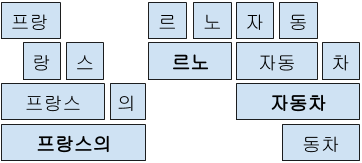
\includegraphics[width=0.5\linewidth]{KoreanLattice}
	\caption[Token Lattice]{A sample lattice showing possible tokenizations of three words of Korean, excluding spaces. The correct selection is shown in bold.}
	\label{latticediagram}
\end{figure}

If we set aside the issue of transducing phonetic data into discrete phonemes, however, the problem of identifying logical groups in a stream of discrete lower-level symbols still remains, and we can isolate this aspect of the problem by working with written text, assembling morphemes and words from a stream of graphemes. In general, tokenization of written text\footnote{In corpus studies, ``text" is often used to refer to any reification of language, be it spoken or written; here however, I will assume that ``text" refers only to written communication.} may be a harder problem than tokenization of speech since writing generally does not reflect spoken language losslessly, and fewer boundary clues (such as prosodic information) will be available. Nevertheless, the fact that reading is possible is itself proof that text-only tokenization can be done at useful levels of accuracy.

\section{Tokenization of English}
In English and many other languages, the problem of text tokenization is often considered trivial: simply split words on whitespace, which substitutes for many of the prosodic clues available in speech. Aken~\cite{aken11}, for example, studied the problem of tokenizing continuous English text with spaces removed, but only as a proxy for understanding human tokenization strategies more generally. While often good enough, however, the space-splitting approach is far from perfectly accurate. Even with perfectly clean data, this approach fails to account for:
\begin{enumerate}
	\item Word boundaries that correctly occur in the absence of whitespace (e.g., before punctuation, with specialized items like URLs, or simply due to typographical errors)
	\item Whitespace that may not indicate a relevant boundary in certain applications (e.g., spaces in compounds, idioms, and borrowed foreign-language phrases used as single logical lexical units).
\end{enumerate}
These complications can be dealt with in various ways, but only on an individual language-by-language basis. Even among languages that all use the Roman alphabet, significant differences in whitespace and punctuation conventions exist. The tokenization conventions for the Penn Treebank, for example, separate ``most punctuation"~\cite{treebank}, but depend on prior knowledge of sentence boundaries to help disambiguate final periods from periods indicating abbreviations and on English-specific knowledge about the structure of contractions and cliticized forms.

Aken's system relies purely on statistical information available within a single text to infer word segmentation. In particular, it keeps track of recurring sequences that occur with frequency greater than a certain threshold as possible word types. It further keeps track of the transition probabilities between known sequences to determine the optimal path through a lattice of tokenization hypotheses~\cite{aken11}. This algorithm was tested against both randomly generated strings of words from a dictionary, and a small sample of natural English text, which revealed a weakness in identifying boundaries in sequences of multiple short words, such as ``in a"; this is a particular weakness shared by other statistical algorithms as well. This approach taken in isolation would likely perform poorly on a text containing a large number of hapax legomena\footnote{types which occur exactly once in a corpus}, which would pass the frequency threshold for recognition, making it potentially less suitable for languages with extensive productive morphology.

Aken's algorithm also depends on an implicit assumption about what the definition of a ``word" is: a fixed sequence of symbols that can occur multiple times. While this assumption may indeed be a useful one for vocabulary induction from unlabeled data, it is not necessarily the best definition of ``word" for all circumstances, especially across multiple languages. Additionally, there is ambiguity in the usage of ``word" to refer to a particular sequence of symbols, versus a particular instance of that sequence in a text. Unfortunately, per Islam~\cite{islam07}, no widely accepted definitions for what constitutes a ``word" exist, even within a single language, let alone cross-linguistically. Different native speakers often segment text in different ways, and the rate of agreement between human judges can be less than 80\%, making it impossible to construct a single ``gold standard" to evaluate results between systems that employ different conventions, whether implicit or explicit. For these reasons, it is often useful to dispense with the problem of defining a ``word" at all and, when exactness is required, to instead refer to \textit{types}, meaning specific abstract sequences of symbols, and \textit{tokens}, meaning specific instances of a type at specific locations in a text. Tokenization is thus the process of identifying meaningful tokens, however ``meaningful" is defined for a particular application in a particular language, and may cover items traditionally identified as ``words" as well as clitics, punctuation, and other errata. Note, however, that differences in conventions regarding what constitutes a meaningful token at a given level of analysis still require consideration during evaluation. The performance of tokenization algorithms is usually evaluated in terms of \textit{precision} and \textit{recall}; precision ($P$) is defined as the proportion of items in the output that are correct (i.e., which match items in the answer key), while recall ($R$) is defined as the proportion of correct items (i.e., entries in the answer key) which are in the output. Mathematically, these are given by
\begin{center}
	$P = \frac{\abs{O \cap K}}{\abs{K}}$ \\
	$R = \frac{\abs{O \cap K}}{\abs{O}}$
\end{center}
where $O$ is the set of output items and $K$ is the set of answer key items. Since it is often easy to obtain high performance on either measure individually (e.g., perfect recall can be achieved simply by guessing that every character boundary might be a token boundary), but difficult to achieve high performance on both, an additional measure, the \textit{F-score} is used to combine precision and recall and provide an estimate of overall performance. In this thesis I use the usual definition:
\begin{center}
	$F = \frac{2PR}{(P + R)}$
\end{center}

While his algorithm requires no prior knowledge of linguistic structure, Aken~\cite{aken11} does note that ``A shortcut [...] is to incorporate a ready-made dictionary that contains some or all of the words that the algorithm will encounter." This lexical-access approach is most clearly demonstrated by Norvig~\cite{norvig14}, who describes the use of a simple lexicon to recursively split a string into a known word and a suffix of remaining characters, using dynamic programming techniques to construct a lattice to avoid the inefficiency of recomputing overlapping segmentations for the same suffixes multiple times. Word-level n-gram frequency data is then used to extract the highest probability tokenization from the lattice. Norvig~\cite{norvig14} cites applications to Chinese, as well as to specialized genres of English, such as URLs, which are written without spaces as previously described.
Norvig's algorithm, however, is only as good as the dictionary\textemdash it will fail on encountering out-of-vocabulary (OOV) words. This makes it less suitable for application to languages that have extensive productive morphology, such as Turkish, in which it may be literally impossible to encode the complete set of possible words in a finite dictionary, even before we account for the fact that new words appear constantly in living languages~\cite{islam07}. Although this overlaps somewhat with the weaknesses of Aken's algorithm, the potential benefits of a hybrid approach are already evident, as a strong statistical algorithm may make up for gaps in vocabulary.

\section{Orthographies Traditionally Lacking Whitespace}
Most practical work in text tokenization involves languages whose writing systems traditionally have no spaces or other written word breaks, such as Chinese, Japanese, or Thai. In these cases, as with the special rules for Treebank annotation, researchers develop separate tokenization systems on a per-language basis, often using substantially different approaches ~\cite{peng04}\cite{suzuki00}.

Peng, Feng, \& McCallum~\cite{peng04} developed a system for Chinese segmentation which recasts segmentation as a tagging problem using linear-chain conditional random fields (CRFs); every character is tagged as either a start-of-word character, or not. This is an inherently hybrid system, as the CRF models incorporate lexical knowledge in addition to lower-level statistics, which are used for probabilistic new-word detection. This provides the best of both worlds: the efficiency and accuracy improvements that lexical access entails, without the need to store the entire vocabulary, and allowing for the proper identification of unknown words as long as they do not exhibit structural characteristics too far removed from those used to create the statistical model (i.e., the normal morphographological\footnote{the written parallel to morphophonological} structure of the language). Their model produced results ranging from ($P = 0.828$, $R = 0.870$, $F = 0.849$) to ($P = 0.953$, $R = 0.961$, $F = 0.957$) over eight tests on various corpora.

The state-of-the-art Japanese segmentation system by Kudo, Yamamoto, \& Matsumoto~\cite{kudo04} also makes use of CRFs to simultaneously achieve tokenization and morphological analysis by selecting the best path through a lattice of possible \textit{morpheme}-level tokenizations generated from a morphologically-aware dictionary. In fact, Kudo et al. were primarily motivated by the problem of morphological analysis of unlabelled text, for which automatic tokenization was merely an unavoidable first step when working with Japanese orthography. This builds on prior work by Asahara et al.~\cite{asahara00} and Uchimoto et al.~\cite{uchimoto01} on Japanese tokenization and morphanalysis using two different statistical modelling techniques: HMMs and Maximum Entropy Markov Models (MEMMs), respectively. Kudo et al.'s CRF model improved on both HMM and MEMM models due to the ability of CRFs to make use of a wider range of tagging features, including lexical information, providing additional evidence for the utility of hybrid segmentation approaches. They report results of ($P = 0.9904$, $R = 0.98.88$, $F = 0.9896$) and ($P = 0.9903$, $R = 0.9920$, $F = 0.9911$) on two different corpora.

Choosing to work at the level of morphemes rather than words additionally removes many of the problems present in other systems with hapax legomena or OOV words. This requires, however, either the ability to re-synthesize complete words from morphemes, or an agreement with later stages of the NLP pipeline to define ``tokens" at the appropriate sub-word level. Where possible, however, the ability to achieve simultaneous tokenization and morphanalysis substantially improves efficiency and provides more contextual information to later stages of an NLP pipeline, such as syntactic parsing.

Suzuki, Brockett, and Kacmarcik~\cite{suzuki00}, in fact, took this one step further, by using a syntactic model to simultaneously select an optimal tokenization while producing a syntactic parse. Like Kudo et al.~\cite{kudo04}, Asahara et al.~\cite{asahara00} and Uchimoto et al.~\cite{uchimoto01}, they also use a ``word breaker" that performs simultaneous morphanalysis while producing a lattice of possible tokenizations. However, they eliminate the complication of collapsing the information in the lattice into a single unambiguous best token sequence. Instead, the lattice is used as the bottom level of a parsing chart, with the selection of the correct token sequence being a natural consequence of identifying the best syntax tree. They report results ranging from ($P = 0.974$, $R = 0.980$, $F = 0.977$) to ($P = 0.981$, $R = 0.985$, $F = 0.982$) on three corpora.

% I thought about adding references to ``Incremental Joint Approach to Word Segmentation, POS
% Tagging, and Dependency Parsing in Chinese", but it doesn't really cover anything new that's
% missing from any of the existing references, and I don't want to focus too much on Chinese
% when I'm not actually doing anything with Chinese.

In my own previous work~\cite{kearsley13}, I addressed the problem of efficient lattice generation with simultaneous morphanalysis using a finite-state transducer (FST) based on the KIMMO two-level morphology system~\cite{koskenniemi84}. This system runs in amortized constant time per-character. Hence, as each input character needs to be examined exactly once and in document order to determine which morphemes it could participate in, it generates a lattice of all possible sequences of known morphemes that could be extracted from an input stream in amortized linear time over arbitrary sized inputs~\cite{kearsley13}. Storing the lexicon as a finite-state transducer both saves a great deal of space and also allows recognition of a potentially infinite number of regularly derived or inflected words, though with some reduction in flexibility versus the CRF models. Compared to a fixed lexicon as used by Norvig~\cite{norvig14}, a morphological transducer suffers less from from the problem of encountering OOV tokens, but does not solve the problem completely; it will still encounter difficulty with unknown roots and other morphemes. This system was tested on English and Turkish, using synthetic corpora consisting of randomly-generated sequences of concatenated words, similar to the method used by Aken~\cite{aken11}. On corpora of known words, the system achieved ($P = 0.209435$, $R = 1$, $F = 0.346335$) for English and ($P = 0.164989$, $R = 1$, $F = 0.283246$) on Turkish.  The low precision scores are attributable to the fact that I focused only on lattice generation, as a clearly separate issue from path selection\textemdash an approach I continue in this thesis. Prior to optimal path selection, the precision measure of a lattice generation system reflects the level of genuine morphological ambiguity present in the input.

The great advantage of this approach is that nearly any morphological model can be adapted to use in a simultaneous lexical-access based tokenizer (although it is optimized for FST-based models). In other words, the language model does not need to be developed with tokenization specifically in mind, and existing analyzers are reuseable, potentially saving a great deal of effort that would otherwise go into another bespoke, language-specific tokenization system. Additionally, this approach specifically supports on-line, real-time usage. While that feature is common (nearly obligatory, in fact) for speech processing, it is relatively rare in text tokenization~\cite{aken11}. On-line operation significantly restricts the types of algorithms that can employed in tokenization, because it is necessary for the speed of processing to keep up with the speed of input. This means that any system intended for on-line use must take, on average, constant time to process each character in the text, resulting in amortized linear ($O(n)$) time to process a complete text. Real-time applications introduce slightly stricter constraints on the maximum allowable constant factor per character.

%NOTE: Plot over p. 8 last & lines?

\section{Psychological Modeling}

In addition to the NLP-oriented approach, the tokenization problem also arises in language acquisition: When hearing a new language that one does not know, how does a learner begin to identify new words to add to their mental lexicon? This clearly requires some generic mechanism (although of unknown and possibly great computational complexity) for inducing probable words boundaries (where contiguous sequences between two boundaries then constitute words) from unlabeled input. That humans are capable of this provides an existence proof of the technical possibility of language-agnostic tokenization.

While studying the ways that human minds may tackle tokenization is not guaranteed to produce the best possible artificial tokenization system since they may involve unnecessary complexity or require quantities of data infeasible to obtain for many NLP applications (in the same way that the best way to build an airplane is not to exactly copy a flapping bird's wing), studies of human psychological segmentation mechanisms do serve two useful purposes: They set a baseline against which errors can be measured, and they may provide an initial example implementation from which further engineering can draw~\cite{daland09}.

To establish a baseline of performance, it is sufficient to use manually-tagged corpora as a gold standard to test against; to provide an example implementation for re-engineering, it is important to have a reasonable psychological model of human speech segmentation. Daland~\cite{daland09} argues that both statistical predictive mechanisms and lexical access are necessarily involved in human segmentation, with contributions from each shifting over the language acquisition process: statistical mechanisms in order to guess at the boundaries around new unknown words and to determine the probability that a potential bounded sequence is in fact a new word, and lexical access to filter errors. Empirical evidence for the validity of this claim is provided by Islam~\cite{islam07}, who reports that many state-of-the-art NLP systems do in fact use hybrid approaches. Daland~\cite{daland09} further proposes that there are only two feasible error-correction conditions for the human tokenization system. The first is statistical over-recognition, where lexical access must filter out erroneously predicted word boundaries; the second is statistical under-recognition, where lexical access must be prepared to add statistically unlikely word boundaries. Logically, however, both may occur in any newly-developed system.

In either case, we can expect an improvement from merging statistical and lexicon-based methods. The set of correct word boundaries found by either method would not a priori be expected to form a subset of those found by the other; thus, their unions would be a larger set of correct boundaries. However, in the case of statistical under-recognition, we would expect a smaller contribution from statistical boundary prediction to the recognition of unknown words by lexicon-based methods. We would thus expect that statistical over-recognition would be the norm, and indeed, this is exactly the result obtained by Rytting~\cite{rytting04}.

\section{Simplified Statistical Models}

Revisiting the analogy of the airplane versus flapping bird wing, one is led to wonder whether statistical models might exist which are much simpler than CRFs or HMMs yet still in some sense ``good enough".  Brent \cite{brent99}, motivated, like Daland, by the study of first language acquisition, identified distribution regularities at the phoneme (or grapheme) level, such as segment-to-segment transition probabilities, to be useful indicators of word boundaries~\cite{brent96}. In later work, Brent~\cite{brent99} and Rytting~\cite{rytting04} both investigated simple character-level statistical cues that could be used as effective predictors of word boundaries during language acquisition, and for tokenization of text. The identification of such useful ``minimal information" predictors holds significant promise for developing simplifications of Daland's cognitive model~\cite{daland09} and further improving the performance of hybrid tokenizers.

While Brent~\cite{brent99} assumed that a prediction technique based on local comparisons (i.e., looking for significant differences between the values of a given statistical measurement between adjacent positions in the text), would be \textit{most} appropriate for identifying word boundaries, Rytting~\cite{rytting04} argued that this is guaranteed to under-predict due to the impossibility of correctly identifying common single-segment words, since the values of any two measurements in immediately adjacent positions cannot simultaneously be either significantly greater than or significantly less than each other. This echoes the problems with identification of small words encountered by Aken~\cite{aken11} with a significantly more complex model. Global comparisons are therefore needed to ensure maximum recall of correct boundaries.

Rytting~\cite{rytting04} tested the predictive power of two statistics based on Brent's work~\cite{brent99}: character-level transition probabilities, and character bigram mutual information scores, using both local and global comparisons for each. Rytting ~\cite{rytting04} showed that, on Greek text, a very simple mutual-information (MI) model outperformed the competing transition-probability models. He also showed that it was highly over-predictive on its own, and that using a global threshold for comparison was the most effective of the techniques that he tested, giving results of ($P = 0.439$, $R = 0.544$, $F = 0.486$) for identifying individual token boundaries. This is despite the fact that the threshold value of zero used in Rytting's study~\cite{rytting04} was chosen ``arbitrarily" with no justification attempted. Rytting's model, however, does also take into account the probability, based on a pre-annotated training corpus, that any particular bigram spans a known word boundary.

In my own previous work~\cite{kearsley14}, I applied the MI approach to English, testing the sensitivity of the model to the quantity of training data available for calculating bigram MI scores. In contrast to Rytting's supervised approach, however, I employed a further simplified, completely unsupervised algorithm which relied solely on MI scores calculated from the unannotated text of the Open American National Corpus (OANC) \cite{oanc}, consisting of samples from a variety of genres including transcribed speech, fiction, news, and technical writing. Additionally, in response to Rytting's claim that the zero threshold is ``arbitrary", I compared its performance with an alternative ``gap threshold" assignment method. In this approach, a model-specific threshold is dynamically selected by dividing bigrams into two clusters based on the largest gap between successive MI scores.

While the results are not directly comparable since our experiments involved different languages, the unsupervised zero-threshold MI approach had better precision than Rytting's supervised approach~\cite{rytting04}, although it comes at a cost in recall\textemdash($P = 0.564$, $R = 0.386$, $F = 0.458$). The gap-threshold approach, on the other hand, showed high recall, but significantly lower precision\textemdash($P = 0.275$, $R = 0.846$, $F = 0.415$). I also found that, above a certain relatively small minimum size, results were not strongly dependent on the size of the training corpus. This, combined with the demonstrated efficacy of the unsupervised approach, means that the data required to build useful statistical word boundary prediction systems can be acquired cheaply, without the need for human annotation. Neither my nor Rytting's results, however, show recall scores close to 1.0, which, together with the early performance plateau, supports Daland's thesis that human tokenization must transition from primarily static-based to more lexical-access based methods during the learning process. While these extremely simple systems based on a single statistical measure (in this case, mutual information) do not have sufficiently good performance to use entirely on their own, their improvement over a random baseline is sufficient to justify investigating their use as heuristic filters to improve the performance of more complex hybrid word segmentation systems~\cite{kearsley14}.

\section{Path Selection Methods}
While my work sidesteps the problem of path selection, it is worth briefly reviewing what options are available. Suzuki et al.'s~\cite{suzuki00} parser-based approach, while highly effective, is also very heavyweight, and several simpler options exist for modular systems that separate lattice generation from path selection. Kudo~\cite{kudo04}, as justification for the need to incorporate lexical knowledge, cites accuracy of over 0.9 using a simple longest-prefix matching algorithm, which simply assumes that the longest prefix of a string which is a known token is a correct token, and then restarts after that longest prefix to find the next token. It is unclear, however, whether the cited statistic applies only to Japanese, or cross-linguistically. Islam~\cite{islam07} also describes a ``maximal match" algorithm (with several variations for resolving ambiguities), which essentially consists of finding the longest substring that is a known token (regardless of whether or not it is a prefix of the text), and then proceeding to select the next longest known tokens in the remaining non-overlapping sections of text. Their particular modification, using type frequency and entropy measurements to resolve ambiguity between equal-length options, achieved ($P = 0.8992$, $R = 0.9469$, $F = 0.9224$) in tests on the Brown corpus. This method is particularly useful in restricted settings where it is necessary to identify correct instances of certain types in desegmented text, but where complete tokenization and identification of unknown tokens is unnecessary; for example, a ``maximal match" algorithm is used in the TIARA\footnote{The Interactive Annotated Reader Application} \cite{cloe12} and Ayamel \cite{todd14} software developed by BYU's ARCLITE Lab in order to identify words and phrases that require annotations to be applied\textemdash an application in which normal English tokenization conventions are completely unsuitable, as the relevant tokens are often large than single words and may contain spaces.
%I know of other instances where this is used for essentially the same purpose, but I'm not certain if I'm allowed to cite them or not due to NDAs
Norvig~\cite{norvig14} provides an approach which incorporates language-specific knowledge but is still relatively simple, calculating the most likely lattice traversal using n-gram probabilities, as noted above. Accurate results from this approach, however, depend on access to an extremely large training corpus (over 3 billion words in this case) to ensure that accurate statistics are available for all possible n-grams; the algorithm's performance is compromised when presented not merely with OOV tokens, but with previously unseen sequences of known tokens. The OOV token problem is partially addressed by model smoothing\textemdash assigning a small default probability to any unknown token\textemdash but can be significantly ameliorated by replacing the simple word n-gram model with a part-of-speech (POS) tag model, which can produce accurate statistics with a much smaller training corpus, since one tag sequence equates to several concrete word sequences. The tag-based approach is particularly attractive for use with systems that employ simultaneous morphanalysis, since POS information comes essentially ``for free".

\section{Lattice Generation with Morphology \& Statistics}

Regardless of the path selection algorithm used, the final results are only as good as their input. If a lattice generation step cannot produce all of the correct token boundaries as hypotheses, then no selection algorithm can produce the complete correct token sequence. On the other hand, a na\:ive conservative lattice generation algorithm could simply propose \textit{every} character boundary as a possible token boundary, in which case the correct sequence is guaranteed to exist somewhere, and could be found\textemdash but only in a highly inefficient manner, as the lattice generator has provided no useful information to guide the search. A separate lattice generation algorithm can thus be rated both on how many correct hypotheses its output contains, and on how much work it requires of the succeeding path selection algorithm. In this context, lexicon-based tokenizers have an additional advantage over many pure statistical algorithms in that they inherently produce pairs of starting and ending boundaries for specific tokens; this significantly reduces redundancy compared to single-boundary tagging systems~\cite{kudo04} like those of Peng et al.,~\cite{peng04}, Brent~\cite{brent99}, or Rytting~\cite{rytting04}. In the worst case, these systems can require considering a number of token hypotheses proportional to the square of the number of individual boundary hypotheses, significantly slowing down the tokenization process.

Based on my previous work, I have built a series of hybrid lattice-generation systems implementing fundamentally language-agnostic lexical-access based and simple statistical algorithms, employing pre-existing morphological analyzers to provide language-specific lexical knowledge. I will show that these relatively simple models produce good results which improve on the performance of either lexical-access based or simple statistical methods alone. I will also demonstrate the generalizability of these algorithms across multiple languages that are orthographically and typologically (specifically, morphologically) dissimilar.